\documentclass[12pt,  a4paper]{report}
\usepackage{graphicx}
\usepackage{booktabs}
\usepackage{chngcntr}
\usepackage{pdfpages}
\usepackage{url}
\usepackage{array}
\usepackage[font=footnotesize]{caption}



\begin{document}

\pagenumbering{gobble}
\def\supervisorIname{Advisor I}
\def\supervisorIIname{Second Reviewer}

	\def\university{Saarland Universitiy}
	\def\institute{Center for Bioinformatics}
	\def\chair{Bachelor's Program in Bioinformatics}
	\def\projectname{MiRNA Target Analysis Using Sequence Alignment}
	\vspace{.2em}  
	\def\author{Louisa Schwed}
	\def\date{September 2016}

\begin{titlepage}

  \begin{minipage}{\textwidth}
    \begin{center}
    { \large Saarland University \\ Center for Bioinformatics\\ Bachelor-Bachelor's Program in Bioinformatics \\}
	\vspace{1.5cm}
    
\includegraphics[width=5cm]{Logo-Universitaet_des_Saarlandes.pdf}\\
    \vspace{1.5cm}
    { \large Bachelor's Thesis\\}
    \vspace{0.5cm}
    {\huge\textbf{\projectname}}\\
    \vspace{1.5cm}
    { \large submitted by}\\
	\vspace{0.5cm}
    {\large\textbf{\author}}\\
    \vspace{0.5cm}
    {\large on September,XX , 2016}\\
    \vspace{1.5cm}
    {\large Supervisor}\\
    \vspace{0.5cm}
    {\large Prof. Dr. Andreas Keller}\\
    \vspace{1.5cm}
    {\large Reviewers}\\
    \vspace{0.5cm}
    {\large Prof. Dr. Andreas Keller}\\
   	{\large Prof. Dr. rer. nat. Eckart Meese}\\
    \vspace{0.5cm}
    \end{center}
  \end{minipage}   
   

\end{titlepage}




\section*{Declaration}
I hereby confirm that this thesis is my own work and that I have documented all sources used. 

\vspace{1cm}

\noindent Saarbr\"ucken, September XX 2016
\vspace{1.5cm}

\noindent Louisa Schwed
\newpage

\newpage

\section*{Acknowledgement}
I would like to express deep gratitude to my advisor, Prof. Dr. Andreas Keller, for his effort and support of my bachelor thesis. Also, I like to thank Prof. Dr. rer. nat. Eckart Meese for his time  to review this thesis. Furthermore, I thank my friends and family for their encouragement and support during my studies and especially throughout the course of this thesis. 

\newpage


\section*{Abstract}

Small endogenous RNAs, called miRNAs, are more and more subjects of investigation because they play an important role in the regulation of gene expression. After a process of maturation they are approximately 22 nucleotides long and target mRNAs by complementary binding. One of the many fields of research on miRNAs is the target prediction. The target prediction is a very complex problem and there is still no perfect solution for it. Many features like base pairing, free energy or conservation for a precise prediction can be incorporated. These features were found by investigation of known target interactions. The database miRTarBase provides a collection of experimentally validated miRNA target interactions. 

In this research paper at hand, I investigate these interactions with sequence alignments. MiRNA and respective target mRNA are aligned and the resulting binding sites are analysed further, especially with regard to how significant the alignment scores are compared to alignments of independent sequences. To analyse the significance of the scores, a negative control is generated by matching miRNAs with random gene sequences. With the help of a t-test and the two samples, p-values can be computed. With these values the significance can be estimated. The result low p-values show a significant increase in the alignment scores of true targets. However, considering the complementarity of the two aligned sequences, no big differences can be observed. The main sequence features, seed region towards the 5' end and additional 3' pairing, cannot be revealed. To get a more reliable prediction, the incorporation of additional features is recommended exemplified by existing prediction tools.
 
\newpage

\tableofcontents

\newpage 
\pagestyle{plain}
\counterwithin{figure}{section}
\counterwithin{table}{section}

\bibliographystyle{apalike}



 
\vspace{1.5cm}

\newpage

\chapter{Introduction}
\pagenumbering{arabic}
\label{chapter:introduction}

miRNAs are small, non-coding RNAs that function in the post-transcriptional regulation of gene expression, especially concerning gene silencing. A miRNA consists of approximately 22 nucleotides which build a single strand RNA \cite{Bartel}. In a process of maturation the miRNA is processed for the actual binding mechanism. The whole maturation of the miRNA is shown in figure~\ref{biogenesis}.\\

In a first step after transcription, the miRNA folds into a hairpin structure and builds the primary miRNA \cite{Lee}. Then, this pri-miRNA is processed by Drosha which results in a precursor miRNA (pre-miRNA). This precursor is about 60 to 70 nucleotides long and contains two single stranded miRNAs. After the export of the miRNA into the cytoplasm another processing step is executed with Dicer to gain the actual form of a miRNA \cite{Lee}. At this stage however, the miRNA is still double stranded and needs to be unwound to be a mature miRNA \cite{Macfarlane}. After processing of the initial double stranded miRNA-duplex, the guide strand will be further used in association with other molecules. In detail, the miRNA is mainly active in combination with a catalytic protein of the AGO protein family. With this protein, the miRNA builds an RNA-induced silencing complex \cite{Ha}. This complex targets a mRNA mainly at its 3' untranslated region (UTR) by complementary binding to the sequence. In this case, the miRNA functions as a guide because its nucleotides pairs with the nucleotides of the target mRNA \cite{Macfarlane}. It can also bind at the 5' UTR or even in the coding region but these are rather uncommon regions. Either way, the binding results in gene silencing either by repression of mRNA translation or degradation of the respective mRNA \cite{Enright}. Which of the two pathways is chosen depends on the degree of complementarity. As figure~\ref{biogenesis} illustrates, if the complementarity is nearly perfect, the target mRNA is degraded. Otherwise, if the seed regions contains mismatches the translation is only repressed and not completely blocked. Both ways have a huge impact on the gene expression. The resulting genetic changes can have consequences like the initiation of cancer \cite{Macfarlane}.\\

\begin{figure}[h]
\centering
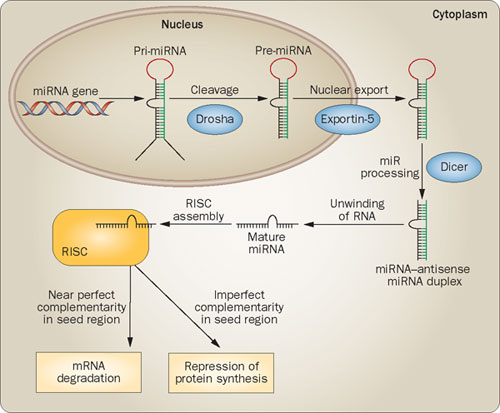
\includegraphics[scale=0.45]{results/biogenesis.png}
\caption{Biogenesis of miRNAs}
\label{biogenesis}
\end{figure}  

The gene regulation by miRNAs plays an important role for many major cell functions like growth, differentiation or metabolism and is currently examined by many researchers \cite{Ardekani}. The importance of miRNA and their regulation mechanism is also expressed by the fact that more than 60\% of all human genes have at least one conserved miRNA-binding site \cite{Friedman}. Therefore, a disregulation of miRNAs, either up- or downregulation, may result on the one hand in different human diseases, e.g. cancer or autoimmune diseases \cite{Ardekani}. On the other hand, this also leads to the assumption that miRNAs could be useful features for the diagnosis and treatment of diseases. However, they follow a very special and complicated targeting and this has to be elucidated. A first step is to understand their function and regulation mechanism. With this information it can be possible to predict targets of miRNAs and then specifically effect these target interactions to diagnose or treat diseases. \\
As already mentioned, especially this prediction of new targets of miRNAs is a major challenge in the whole field of miRNAs. There is still no perfect, reliable solution for it. A few tools exist that try to solve this problem. One of the first tools was miRanda which was developed by Enright et al. In their prediction algorithm they rely on three main features: sequence complementary, free energy and evolutionary conservation \cite{Enright}. Another tool is miRSVR which uses bit vectors and statistical learning approaches to predict targets. In the bit vector information like base complementarity, UTR length and distance, AU content and conservation is stored \cite{Betel}. A third tool was developed by Bartel et al. and is called TargetScan. Their approach is based on seed matching and additional features like UTR positioning, AU content as well as base pairing of the nucleotides 12 or 13 to 16 of the miRNA. They especially take the seed region into account by defining four different patterns of seed binding sites \cite{Lewis}.\\

Because the miRNA binds to the sequence of its target gene an obvious starting point can be the complementarity of the miRNA sequence to the gene sequence as almost each tool considers at first. The first idea could be that if the sequence complementarity of miRNA and target mRNA is relatively high at a certain position, a new target site could be found. With the help of sequence alignments, these regions of high complementarity can be identified. In that case, very high alignment scores could indicate a high probability that there is a true binding site at this position. This alignment could then be used to predict completely new target sites and decide whether the considered mRNAs is targeted by a certain miRNAs. Whether this is a reliable indication or not will be discussed below. For this assumption of using the alignment score as a feature, there already exist some problems beforehand. Since it is known that the main binding happens within the seed region, other regions are not necessarily complementary and this may lower the complementarity and consequently the alignment score. \\

The main feature that most of the tool consider first is the sequence complementarity especially at a certain seed region. In contrast to miRNAs in plants which bind nearly perfectly complementary to their targets, miRNAs in animals bind less tightly and are not perfectly complementary \cite{Rhoades}. There can be regions were the nucleotides are unbound which results in complex secondary structures which are hard to predict \cite{Rehmsmeier}. The main complementary region or seed region includes nucleotides from position two to eight starting from the 5' end. Figure~\ref{seed} shows the scheme of the seed region \cite{Peterson}. \\


\begin{figure}[h]
\centering
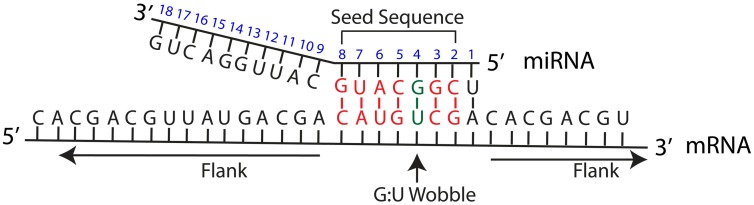
\includegraphics[scale=2.8]{results/seedmatching.png} 
\caption{Scheme of seed matching}
\label{seed}
\end{figure}

The irregularity of the presence of non-complementary regions makes a reliable prediction for animals more difficult than for plants. When concentrating mainly on the seed region for a prediction, it will lead to many false positives. This small region of seven or eight nucleotides would be too unspecific because they can be present by chance in the mRNA although there is no real binding site at this position. It is recommended to take more than the seed region and the sequence complementarity into account to increase the complexity and specificity of the prediction. How significant the consideration of the sequence complementarity of miRNA and mRNA sequence is, will be further analysed with validated data in this research. For theses known interactions of the database the alignment scores are investigated whether these are significantly higher than for miRNA and sequences that are no real targets. Another point that is considered is my own found binding site accord with the ones given in the database that are provided by existing prediction tools. \\


\begin{figure}
\centering
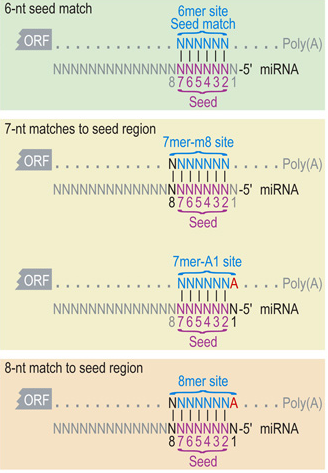
\includegraphics[scale=0.6]{results/canonical_sites.png}
\caption{Canonical sites of seed region}
\label{Fig:canonical}
\end{figure}


In the mentioned seed region there can be different types of matching patterns: perfect matching between six nucleotides starting at the second nucleotide, seven nucleotides including the 8th position, seven nucleotides and an Adenine at position one or eight matching nucleotides from position one to eight and also an Adenine at position one \cite{Grimson}. Figure~\ref{Fig:canonical} illustrates the different types of sites. Grimson et al. investigated the different types of sites referring to the effectiveness of the gene repression \cite{Grimson}. Staying with sequence complementarity, following a region of non complementary nucleotides towards the center of the miRNA, another matching region towards the 3' end can be observed. Aligning miRNA to target mRNA could shed light on the occurrence of this region.  \\



To gain information about targeting and whether and to what extent alignment and sequence complementarity play a role in this process, databases provide reliable data about miRNAs and their targets. 
For these miRNA analyses, there are three main databases that provide the necessary information. A collection of experimental validated miRNA-target interactions(MTIs) is essential. The database miRTarBase provides a big dataset of validated MTIs \cite{Hsu}. To get information about every single miRNA for different organisms miRBase contains large datasets about the miRNAs. The most interesting information is sequences of the precursor and of all mature miRNAs \cite{mirbase}. For further analysis I will only consider miRNAs of \textit{Homo sapiens}. Last but not least, I used the UCSC Genome Bioinformatics Site. In their table browser you can get data files about human gene sequences and untranslated regions and their respective sequences \cite{ucsc}.
  
\vspace{1.5cm}


\chapter{Data and Methodology}
\label{chapter:data and methodology}

 
\section{Data} 
\subsection{miRTarBase}
The database mirTarBase, which was released in 2010, provides by now about 7500 strong validated MTIs and 348000 weak ones from different species \cite{Chou}. One constraint in this research is that I concentrate on humans. Different experiment types were used to validate the data, including Reporter assay, Western plot, qPCR, Microarray, NGS, pSILAC and other methods whereas the first three are the ones that deliver strong evidence. The strong types detect the co-epression of miRNAs and their target gene, more precisely, the mRNA expression levels when miRNA is overexpressed or knocked down  \cite{Hsu}. Another constraint is that I only concentrate on the strong evidence targets. The data collection provides many information about the interaction between one miRNA and its target. Interesting details are the predicted alignments of miRNA and target 3' UTR sequence by either the author of the MTI or other prediction tools like miRanda. These alignments will also play an important role in the following analyses. \\

From the database catalogue the respective MTI data tables of the specific species can easily be downloaded, in this case \textit{Homo sapiens}. The table then contains the following information as also shown in figure~\ref{mirtarbase_scrot}: miRTarBase ID, miRNA name, species of the miRNA, target gene symbol, target gene Entrez ID, species of the target gene, experiment type, support type, references. The fields of interest for the research are name of the miRNA, the target gene ID and the experiment type because I only concentrate on the Functional MTIs that are not weak. That means, every single strong validated interaction was analysed.\\

As mentioned above, the miRTarBase provides also binding sites as alignment positions predicted by different tools. To decide whether the alignments found in this research are compatible with the ones provided, the miRTarBase html page of the single MTI was parsed to get the start positions of each provided alignment. These positions do not exist for every miRNA but for about 3700 of the interactions. The parsed positions can then be compared to the resulting positions by the pairwise2 module. This will be described in detail under section~\ref{sec:meth} Methodology.\\ 

\begin{figure}[h]
\centering
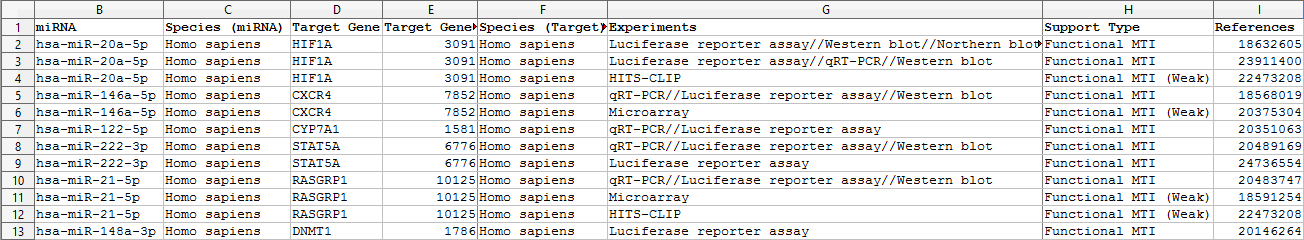
\includegraphics[width=\textwidth]{results/mirtarbase_scrot.png}
\caption{Extract of the miRTarBase file}
\label{mirtarbase_scrot}
\end{figure}
\vspace{0.5cm}


\subsection{miRBase}
To get the corresponding sequence of the miRNA name, miRBase, which was already published in 2005, provides a complete dataset of all known miRNAs \cite{Griffiths-Jones}. By now it contains about 35000 mature forms and 2500 of them are found in \textit{Homo sapiens}. The table with all miRNAs includes the accession number, miRNA ID, status, sequence, accession number of first mature form, its ID, its sequence, accession number of the second mature form, its ID and its sequence. I only use miRNA id and the respective sequences to align those to the gene sequence \cite{mirbase}. Figure~\ref{mirbase_scrot} shows an extractof the file.\\


\begin{figure}[h]
\centering
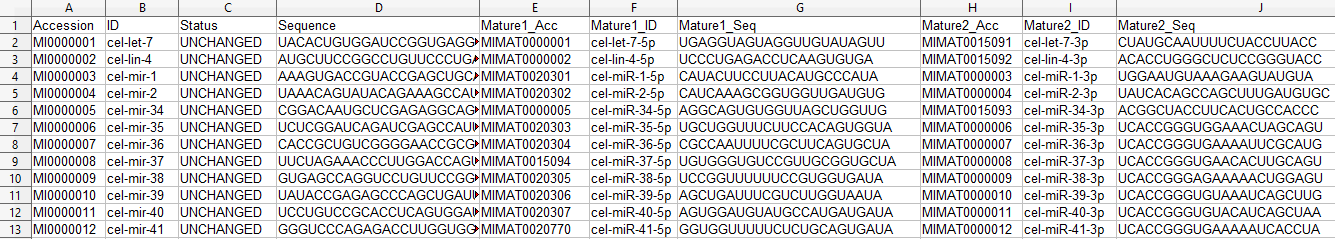
\includegraphics[width=\textwidth]{results/mirbase.png}
\caption{Extract of the miRBase file}
\label{mirbase_scrot}
\end{figure}


\vspace{0.5cm}

 
\subsection{UCSC Genome Bioinformatics Site}
The last required dataset is the collection of target gene sequences and their respective untranslated regions (UTRs). On the UCSC Genome Bioinformatics Site I generated a list of all genes and their UTRs of the human genome using the Table Browser \cite{ucsc}. The selected assembly was Dec. 2013 (GRCh38/hg38) and the track was RefSeq Genes. As an output format I selected the sequence. Next, the sequence type was set to genomic and the regions 5' UTR Exons, 3' UTR Exons and introns were chosen. The reuling list consists of a description of the gene with the transcript accession number (NM-number) and the concatenated sequences of 5' UTR, gene and 3' UTR as shown in figure~\ref{ucsc_scrot}.\\


\begin{figure}[h]
\centering
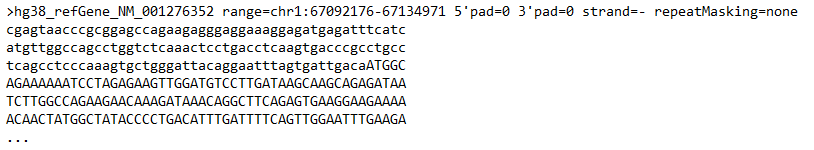
\includegraphics[width=\textwidth]{results/ucsc.png}
\caption{Extract of the UCSC genome file}
\label{ucsc_scrot}
\end{figure}



\subsection{ID converter}
\label{sec:id}
For the alignment of miRNA to the corresponding gene the respective miRNA sequence and gene sequence are required. The interaction data from miRTarBase only provides the correlation between miRNA name and target gene ID. In contrast, the dataset from UCSC only delivers the NM number for the gene sequence. Therefore a conversion from gene Entrez ID to Refseq mRNA accession number is required. Biodbnet provides a conversion tool for different IDs, names and numbers \cite{biodb}. I entered all existing target Entrez IDs of the miRTarBase file and obtained a conversion list of IDs and their corresponding Refseq accession numbers. In my program I used this list by storing every entry in a dictionary and looked up the particular ID for every MTI. This is also described in the following section.
 


\vspace{1cm}


\section{Methodology}
\label{sec:meth}


The program for the analysis is implemented in Python. As input files the UCSC gene file, miRTarBase file and miRBase file are required in a csv format. Additionally the conversion file of gene id and nm number is needed. It can be generated as described in section~\ref{sec:id} ID converter and used as an input file in a text format. 
For each data file, except the MTI file, an own dictionary is generated. Therefore the data files are parsed and each entry is stored into the respective dictionary that allows fast searching. For the miRNAs the dictionary is defined as follows: miRNA name as key and sequence as value. The two mature forms, in case there exist two, are stored separately. For the gene file, the NM number is the key and the value is a list of sequences of 5' UTR, coding region and 3' UTR. At last, for the conversion list, the Entrez id is stored as the key and the list of NM numbers as a value. More than one NM number for one gene Entrez id can exist because different transcripts can be obtained by alternative splicing. \\

Then for every MTI in the miRTarBase file the respective miRNA sequence is searched for in the miRBase dictionary and combined with the gene sequence of the corresponding target in the gene dictionary. The miRTarBase file contains data of 'Functional MTI', 'Functional MTI(Weak)' and 'Non-Functional MTI'. In this paper, I only consider the strong validated data of the Functional MTIs because they deliver strong evidence for the interaction. Hence, if an entry in the miRTarBase file contains something other than 'Functional MTI', it is skipped. \\

After matching miRNA and gene, a local alignment is performed. Therefore, I took the whole gene sequence, meaning the concatenation of UTR and coding region. This will show whether the preferred binding will be within the 3' UTR, as known, or somewhere else. An alignment is defined as the optimal positioning of the bases of one sequence, in this case the miRNA, to a region in the other sequence, the gene sequence. The result reveals functional or structural similarities. \cite{alignment}. In this case, the similarity can be interpreted as region where a binding site could be present. Therefore, if we take the reverse complement of the miRNA sequence and align it to the mRNA sequence, this will simulate the binding. More precisely, if the alignment score is high, the sequences (mRNA and reverse complement of miRNA) are more similar, implying the actual miRNA could possibly bind at this alignment position. Because the miRNA can bind at any region in the gene, a local, not a global, alignment is executed.\\

The Biopython library provides a module, pairwise2, for pairwise local alignments of two sequences. This tool is based on a dynamic programming algorithm. This function can be used either with default parameter or different scores and costs can be defined. The default parameters are as following: +1 for matching character, 0 for not matching ones and there are no gap penalties \cite{pairwise}. To get a more suitable alignment, own parameters can be selected. Table~\ref{table:parameter} shows the different parameters I used to analyse the data. Set no. 8 is similar to the parameters they used for the tool miRanda \cite{Enright}. The other parameters are logically selected to test which influence they have on the results. \\


\begin{table}
\caption{Parameter sets}
\vspace{0.3cm}
\begin{tabular}{c|c|c|c|c}
Parameterset & match score & mismatch score & gap open & gap extend\\
\hline\hline 
1 & default: 1 & default: 0 & -4 & -4\\
2 &  default: 1 & default: 0 & -5 & -1 \\
3 &  1 & -2 & -2 & -1 \\
4 &  2 & -2 & -5 & -4 \\
5 &  3 & -2 & -4 & -4 \\
6 &  5 & -1 & -8 & -4 \\
7 &  5 & -2 & -8 & -3 \\
8 &  5 & -3 & -8 & -2 \\
9 &  5 & -4 & -6 & -4 \\
\hline
\end{tabular}
\label{table:parameter}
\end{table}



For each alignment the following steps are performed: the pairwise2 module delivers the best alignment with the highest score. Sometimes there is more than one alignment because they have the same highest score. For each found alignment list, the miRNA name, the respective NM-number and the alignment score are stored in a string. Then, for each single alignment in the list, the starting position is computed and added to this string. To get a final list of all alignments, the single strings of each MTI is written to a text file.\\

For the analysis of the complementarities, the alignment is further examined. First, both sequences are reversed because they are given from 3' to 5'. To further analyse the 5' seed region and make the plots more clear, the sequences then start with the 5' end. 
Each nucleotide position of miRNA and target mRNA is compared and whenever the nucleotide is the same, a '1' is added to a list, otherwise, if they are different or there is a gap, a '0' is added. This list is yielded to a big matrix for the final analysis. Going through this matrix through each column the number of '1's is computed and divided by the total number of elements in the matrix. The result will be the ratio of complementary bases. This ratio is plotted for each position in the alignment. \\

To be able to analyse the data statistically a set of negative controls is required. To produce this data, 1000 miRNAs of the miRBase file were randomly assigned to a list of genes. Then, this non target file is processed in the same way as the file of the true target interactions. The random assignment can by chance contain true targets but generally the miRNAs are matched with genes that are not targeted by them. \\

For the datasets the average and standard deviation were computed with functions of LibreOffice. A statistical two-tailed t-test for two samples with equal variances was performed with LibreOffice as well \cite{ttest}. In this case, one sample was the data set of the true targets, the other one the data of the non-targets. The t-test function provides a p-value as a result. The lower this p-value is, the more significant the increase of the alignment score of the true targets is. If there is an increase in the score, this would indicate a true target. Hence, if we only calculate the alignment score for a new miRNA and any target sequence and observe a high score, the probability that a new, true target was found would be high. Whether this is a reliable feature for the prediction will be discussed in the following.\\

For the analysis of the alignment starting position, the miRTarBase was parsed first. For each strong validated data in the file the respective miRBase target page was parsed and the three given starting positions were searched. In order to do that, the MTI id was inserted into the url which was opened. Together with the corresponding miRNA name and target NM number the positions were stored in a text file. In the final table the starting positions found were compared to the positions given in the resulting text file what was mentioned before. The final number of positions found is stored in the final result table as well. 



\vspace{1cm}



\chapter{Results}
\label{chapter:results}

For each parameter set the computed alignment score for every MTI is stored in a table. Additionally the average alignment score, the standard deviation and the p-values are listed below. Table~\ref{table:results} shows only a summary of the resulting table of the program, excluding the single alignment scores of each MTI that the program provides. 13934 alignments were computed for the true targets and 2717 for the non-targets. To draw a better comparison, the scores of the non-targets are listed right under the scores of the true targets. The averages of both alignment score sets show that the scores of the true targets are in general only slightly higher than the ones of the non-targets. For the lower alignment scores e.g. of set 1 -2 -2 -1, resulting from really low match scores, the difference is only 0.3, and at first sight not very significant. For the higher scores, the difference amounts to two which is an increase of about 3\% for the parameter set 5 -1 -8 -4. At first sight, it is hard to say if this is significant because the scores are generally higher and therefore the amount of two is not much. \\

The standard deviation of the non-targets is slightly higher than that for the true targets but also not very significant. Hence, the scores of both cases are similarly spread from their means. The p-value sheds light on whether the increase in the alignment score is significant when considering the population of scores. According to the low resulting p-values of the t-test, which were computed as described in section~\ref{sec:meth} Methodology, the increase in the alignment scores is significant. The parameters 5 -1 -8 -4 show the most significant difference with a p-value of 2.529 * 10\textsuperscript{-61} whereas 2 -2 -5 -4 shows the least significant increase but also here the p-value is very low with 3.279 * 10\textsuperscript{-36}. So even though the average scores do not differ by much, the scores of the true targets seem to stem from the higher scores and the ones of the non-targets from the lower scores. Additionally, there are many more scores for the true targets than for the negative control. If the average score is about two points higher for this parameter set, the bigger data set of true targets has to include many more MTIs with higher alignment score to increase it by two. Taking this consideration into account, the amount of two is not that low. Hence, there must be many alignments with higher scores. \\

\begin{table}
\centering
\footnotesize
\caption{Table of alignment results}
\vspace{0.3cm}
{\setlength{\extrarowheight}{5pt}
\begin{tabular}{c|c|c|c}
& 3 -2 -4 -4 & 5 -1 -8 -4 & 5 -2 -8 -3 \\
\hline\hline
Average true targets & 33.096 & 64.247 & 59.495	\\
Average	non-targets & 31.831 & 62.199 & 57.464 \\
\hline
Standard deviation true targets & 4.058	& 5.758 & 6.304\\
Standard deviation non-targets & 4.233 & 6.510 & 6.753 \\
\hline
t-test p-value & 5.934 10\textsuperscript{-49} & 2.529 10\textsuperscript{-61} & 1.040 10 \textsuperscript{-51} \\\hline
\end{tabular}}\vspace{0.5cm}

{\setlength{\extrarowheight}{5pt}
\begin{tabular}{c|c|c|c}
& 5 -3 -8 -2 & 5 -4 -6 -4 & -4 -4 \\
\hline\hline
Average true targets & 56.391 & 55.510 & 13.712 \\
Average	non-targets & 54.269 & 53.294 & 13.362\\
\hline
Standard deviation true targets & 6.633 & 6.806 & 1.078\\
Standard deviation non-targets & 6.876 & 7.01 & 1.311\\
\hline
t-test p-value & 1.394 10\textsuperscript{-51} & 1.744 10\textsuperscript{-53} & 8.824 10\textsuperscript{-50} \\\hline
\end{tabular}}\vspace{0.5cm}


{\setlength{\extrarowheight}{5pt}
\begin{tabular}{c|c|c|c}
 & -5 -1 & 1 -2 -2 -1 & 2 -2 -5 -4  \\
\hline\hline
Average true targets & 13.710 & 8.593 & 18.351\\
Average	non-targets  & 13.361 &	8.208 &	17.619 \\
\hline
Standard deviation true targets & 1.078	& 1.347	& 2.751\\
Standard deviation non-targets & 1.309 & 1.385 & 2.868\\ 
\hline 
t-test p-value & 1.13110\textsuperscript{-49} & 8.157 10\textsuperscript{-42} & 3.279 10\textsuperscript{-36} \\
\hline
\end{tabular}}
\label{table:results}
\end{table}



Another observation is that the difference between the parameters is not that big. For each set, the increase is still very significant, even though the p-values range from 10\textsuperscript{-36} to 10\textsuperscript{-61}. There is no exception that does not show significance in the alignment scores of the true targets. The differences in the value of the scores in general are obviously a result of the different match and mismatch scoring and penalizing gaps which can be more or less. A certain penalty for gaps should be present because it is not very logical from a biological sight that the alignment contains many gaps. This alignment as described above should simulate the binding to the target binding site. If a miRNA binds to its target, it binds with some regions of complementarity as well as with some bulges. However, a binding with too many bulges is not common and the regulation would not function very well. Therefore few gaps are sensible but many and longer ones should not be present.
The parameter set with the highest p-value has low match and mismatch scores compared to the gap costs. So gaps are more penalized than mismatches. This will result in binding sites with less gaps and some mismatches. The complementarity of the true targets will therefore be lower and the binding site will not be very specific. Analysing the non-targets, they should not have true binding sites because they are randomly assigned to miRNAs. Therefore, aligning these two sequences should generally result in worse binding sites where the complementarity is as well not very high. Comparing them to the true targets which have also worse binding sites because of the scoring, the difference between the two groups will not be very high. And this can be seen in the higher p-value. Nevertheless it is still significant. \\


\begin{figure}
\centering
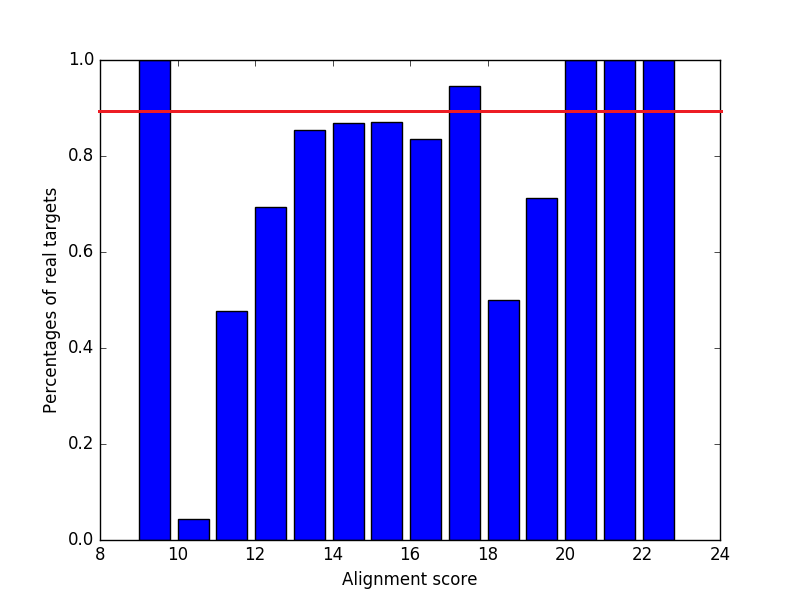
\includegraphics[scale=0.28]{results/plot_scores-4-4_thresh.png}
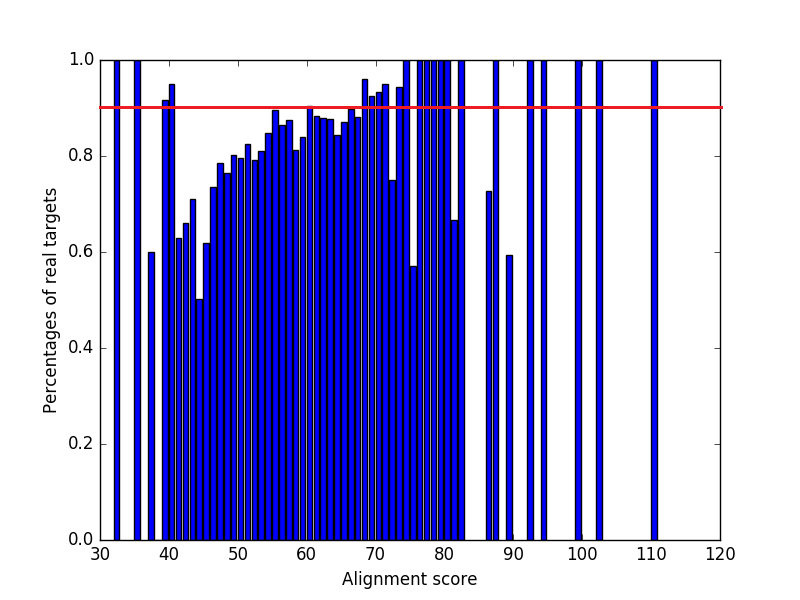
\includegraphics[scale=0.28]{results/plot_scores5-3-8-2_thresh.png}
\caption{Distribution of alignment scores, parameters -4 -4 and 5 -3 -8- 2}
\label{fig:distribution}
\end{figure}

The increase in the alignment score can be also be observed when considering the distribution of the scores within the two groups of case and control. For two parameter sets (No. 1 and No. 8) the distribution was plotted and is shown in figure~\ref{fig:distribution}. On the x-axis the different existing scores of the respective data set are shown and on the y-axis the ratio of true targets that had these scores. It can be observed that towards the higher alignment scores the ratio of true targets rises. But there are some scores that are exceptions because more non-targets produced these scores than true targets, shown by lower y-values. Using this score as a prediction feature, a threshold needs to be determined to identify a true target. Hence, a certain ratio has to be exceeded to rank this score as high enough for being a true target. In figure~\ref{fig:distribution} a threshold of 90\% is delineated meaning at least 90\% true targets produced a certain alignment. Still 10\% of random non-targets had this score as well. Assuming this threshold and using the alignment scores for a prediction the first parameter set shows that if we have scores of nine, 17, 20, 21, 22 or 23, a mRNA would be classified as a true target. On the one hand, obviously the score nine would not fit in the pattern because it is a very low alignment score and the binding site would not be very suitable because there certainly are many mismatches or gaps that lower the alignment score. On the other hand, alignments of miRNA and mRNA with a resulting score of 19 which belongs to the higher scores for this set, would not be classified as a true target even though the binding might be suitable. How this classification will look like strongly depends on this threshold. A lower threshold will result in a lower specificity and higher sensitivity and vice versa for the higher one. The two measurements of the performance need to be balanced and determined depending on the analysis. \\

For the second plot in figure~\ref{fig:distribution} the same can be observed: some lower alignment scores are above the threshold although they are not suitable and for some higher ones the probability to be a true target would be low. But in general it can be said that if the score is above 70, the likelihood that the target is a true target is quite high. In this plot it can also be seen that there are some outliers with high alignment scores. There are very few with rather high scores like 100 and 110 but scores in between the two were not produced, neither by true targets nor by non-targets.  \\

Summing up, assuming the score as the only prediction feature and given a certain threshold, some mRNAs are predicted right to be true targets but there are also false positives and false negatives. Given high scores of the alignment of miRNA seqeunce and mRNA sequence, a mRNA is not necessarily targeted by this miRNA. This uncertainty can be accounted for by considering and combining many more features such as conservation or energies and get a more reliable prediction.\\


\begin{figure}
\vspace{-1cm}
\hspace{-1cm}
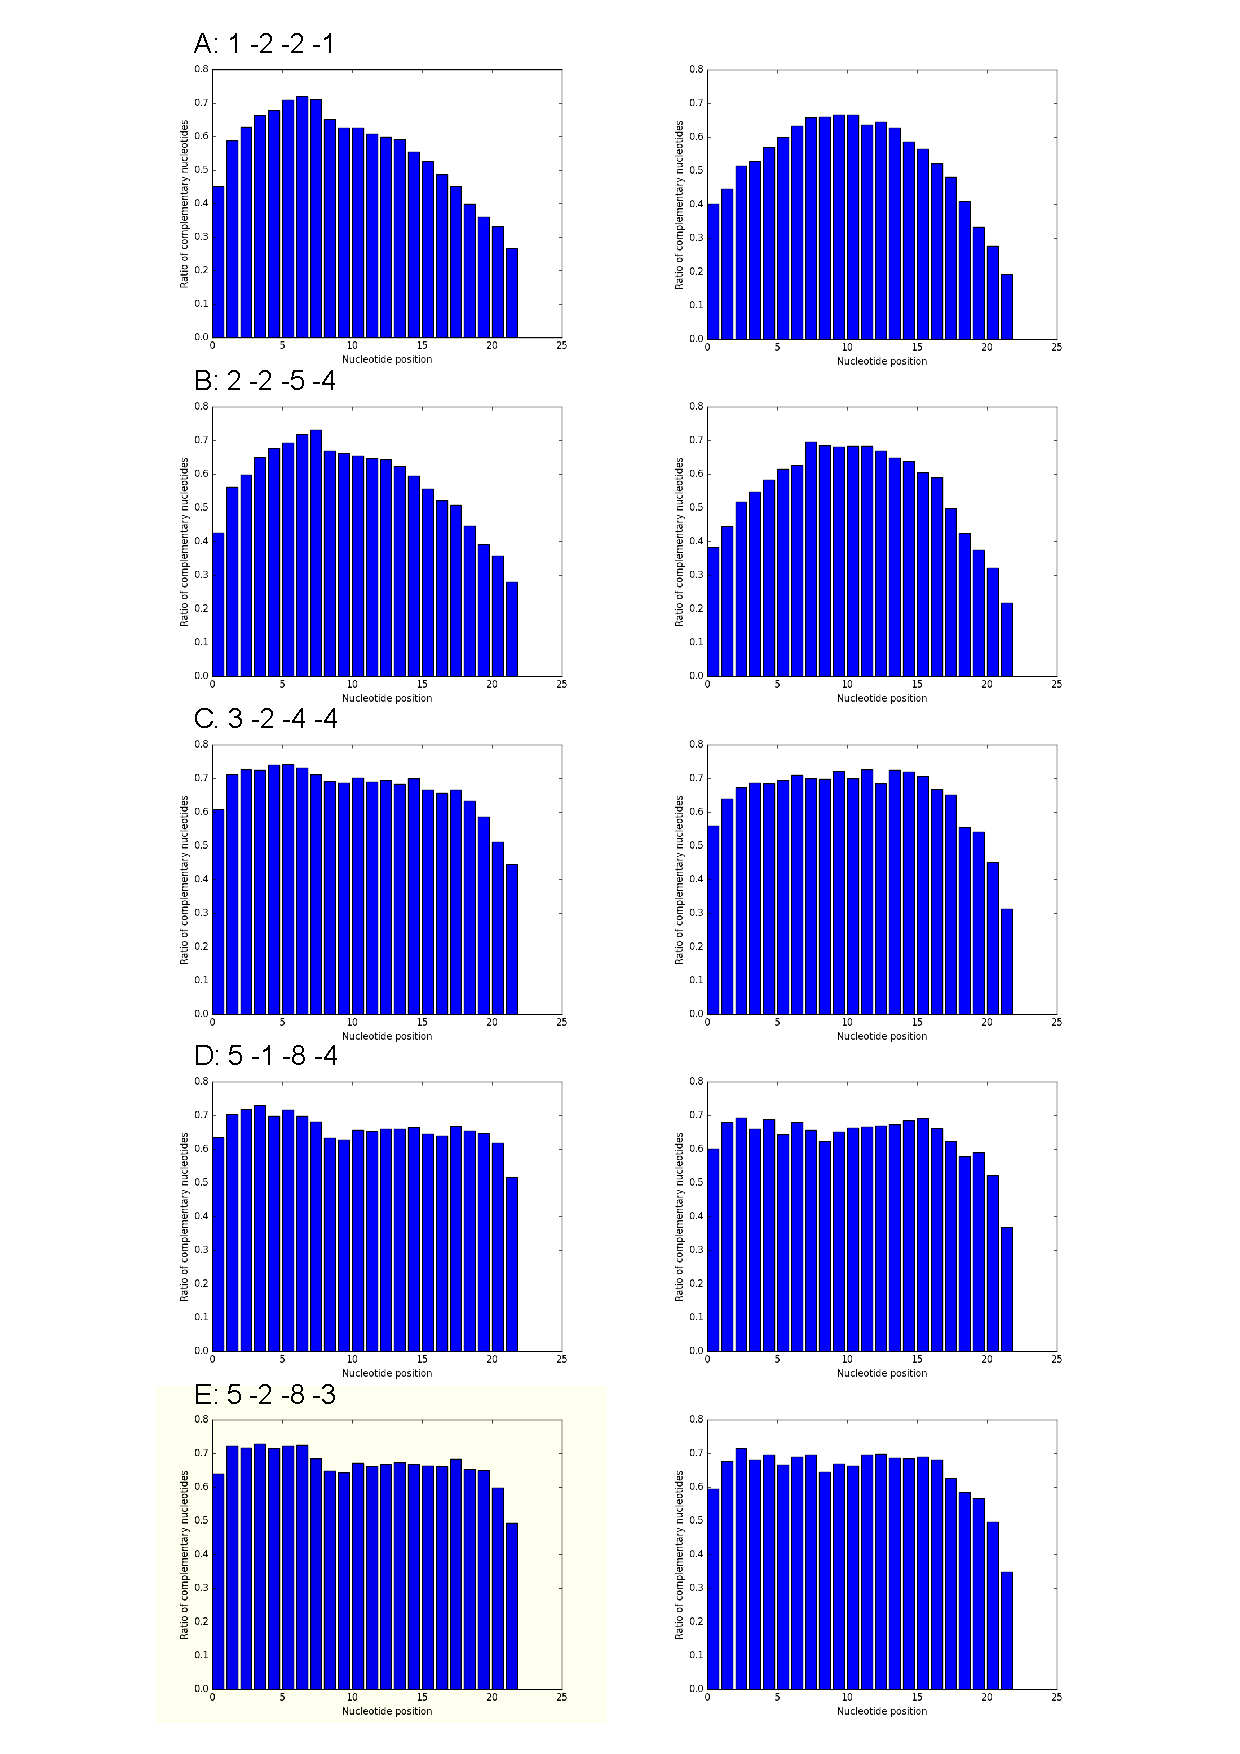
\includegraphics[scale=0.75]{results/compl1.pdf}
\end{figure}

\begin{figure}
\hspace{-1cm}
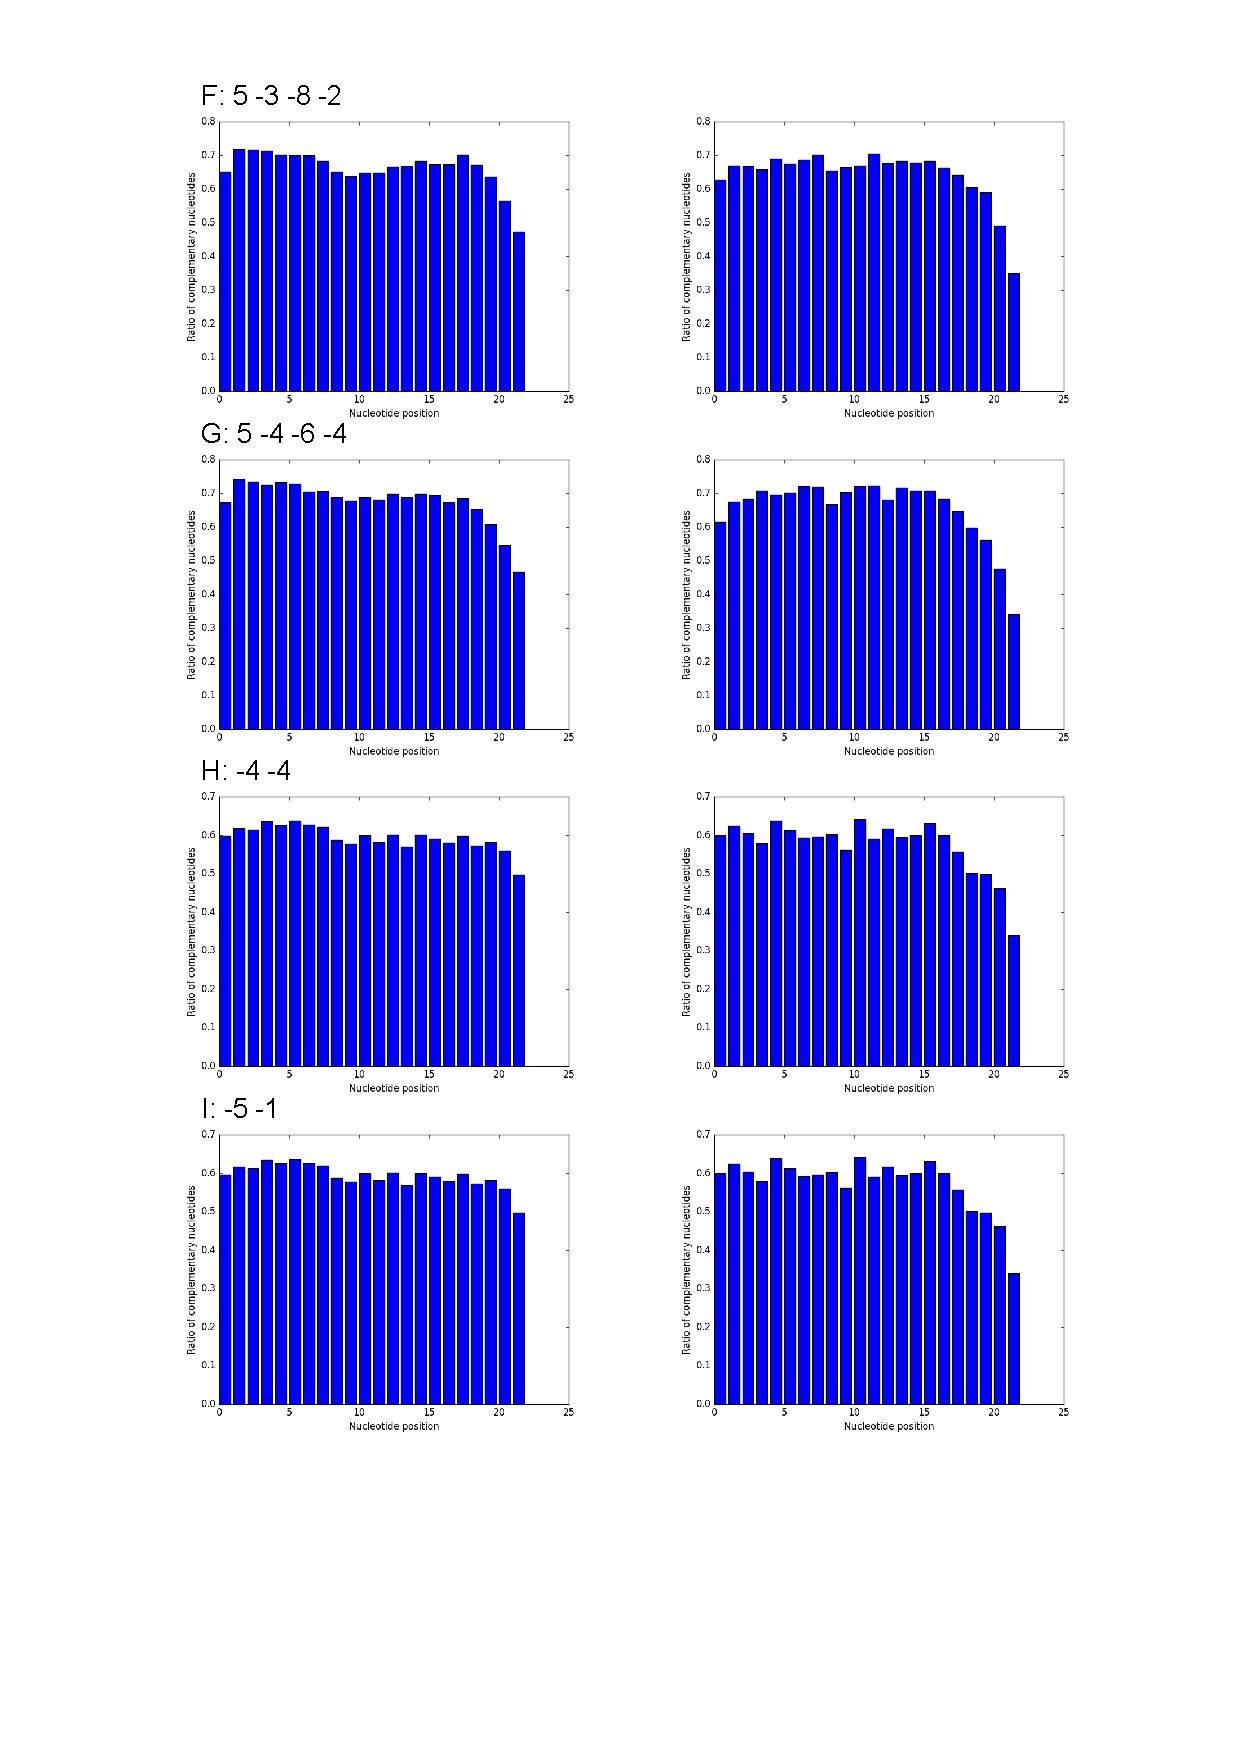
\includegraphics[scale=0.75]{results/compl2.pdf}
\vspace{-4cm}
\caption{Ratios of complementarity per parameter set (A-I): targets left, non-targets right}
\label{ratios}
\end{figure}


As described in the Methodology, for each parameter set the complementarity of the single alignment positions of the miRNA and target gene sequence were plotted. These plots for the different sets are shown in figure~\ref{ratios}. The x-axis of the plots shows the position one to 22 of the miRNA, the y-axis represents the ratio of bases that are complementary at this position, considering all alignments produced with these parameters. Because most of the miRNAs are only 22 nucleotides long, I will only focus on these positions. Higher positions would be very imprecise because of the different lengths. The non-targets are shown on the right site, the true targets on the left.\\

In general it can be seen that the bars of the non-targets are never higher than 70\%. The true targets sometimes exceed this percentage but not very often. For some sets there is a more significant difference between true targets and non-targets than for others. Regarding set A, for the true target left an increase in complementarity in the seed region can be observed. Whereas the first position is below 50\%, the complementarity rises from the second position on to the 8th. The ratio towards the end gets really low down to 30\% of complementary bases. In comparison, the maximum of complementarity of the non-targets right is shifted towards the central positions, not showing the typical seed region. From then on it decreases very fast as well. Notably the plot of the true targets does not show the complementary region towards the 3' end. The same applies for plot B. Although the parameters are very different the plot for the true targets looks similar to that of A. The right plot even more reveals the difference between the two groups. There is again an increase in the positions eight to 13, not fitting into any rule of targeting. \\

Considering the other figures of the complementarities, the seed region is always recognizable, although not very strong. The increase in the first few nucleotides amount only to a few percentages. The plots of the non-targets do not follow any rules as expected. The complementarities are almost constant and drop at the end down to 30\%. For the true targets the decrease at the end can also be observed but not so much. Plot H and I stay almost constant above 50\%.\\

Summing up for the true targets the complementarity is almost as high as for the non-targets, gaining no reliable information for the prediction. This implies that the consideration of the complementarities of the miRNA positions is not a significant and reliable prediction feature. Only having these ratios, it can not certainly be decided whether this plot shows a true targeting or not. \\

In figure~\ref{curves} three plots with curves of three parameter sets illustrate the complementarities of the nucleotides in an alternative way. In the first plot the difference in the seed region can be seen. The blue curve of the true targets is about 10\% higher than the curve of the non-targets. From nucleotide eight on, the red curve declines from its maximum until it crosses the blue one but the difference is not very big. From then on the curves are very similar and they both drop down to 30\%. So for this parameter set only a difference in the seed region can be observed. The second plot of the parameter set 5 -4 -6 -4 shows even less differences. Again, there is a small difference in the seed region where the blue curve is slightly higher but only up to 5\%. Then both curves stay at a high level between 65 and 70\% which is a contrast to the first plot. But the main point, a difference between true and non-targets can not be observed. The last plot is slightly different from the two others. The blue and the red curve alternate and are very similar in height. In this graph, neither seed region nor additional 3' pairing can be observed. Similarly, additional pairing cannot be observed at all for the two other graphs. All in all, the plots and the complementarity of the pairing nucleotides deliver not much information. Concluding, having a look at the complementarity of a new examined binding site is not significant to decide whether this position is a newly found binding site and hence an actual target of a miRNA. \\

\begin{figure}
\centering
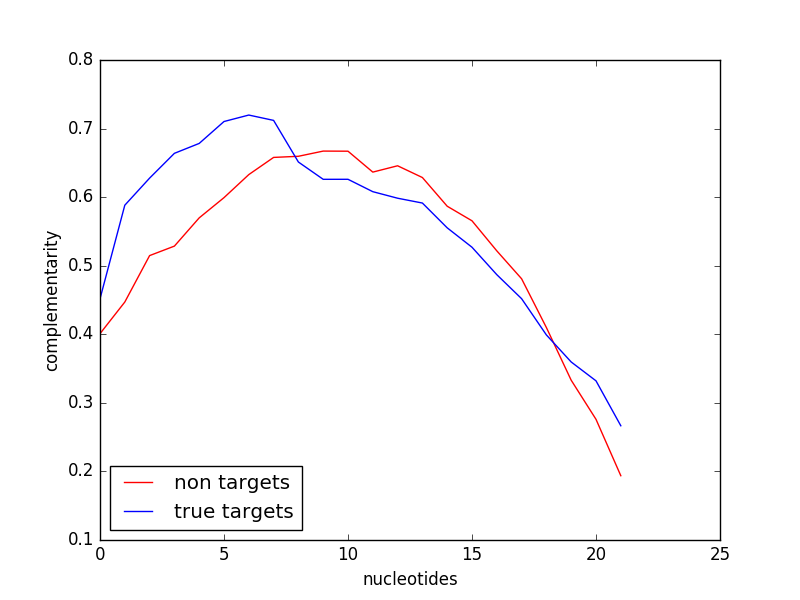
\includegraphics[scale=0.3]{results/curves1-2-2-1_new.png}
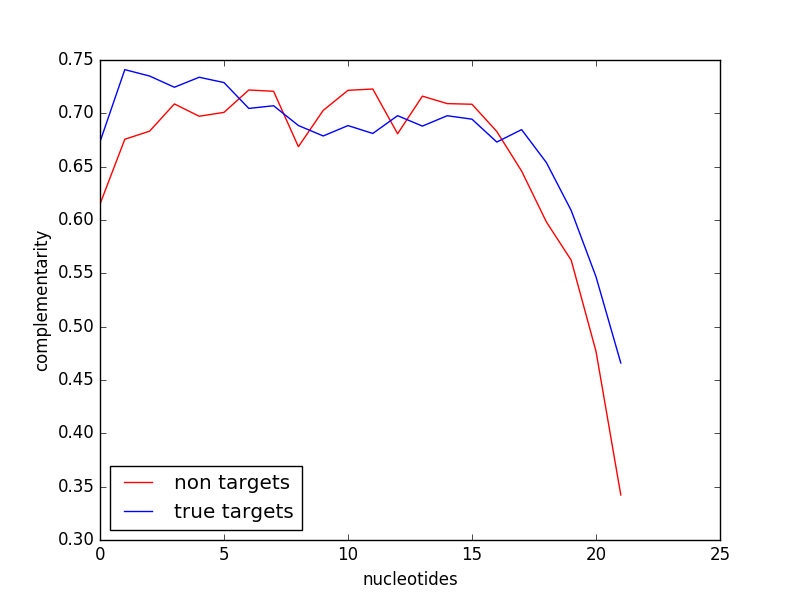
\includegraphics[scale=0.3]{results/curves5-4-6-4_new.png}
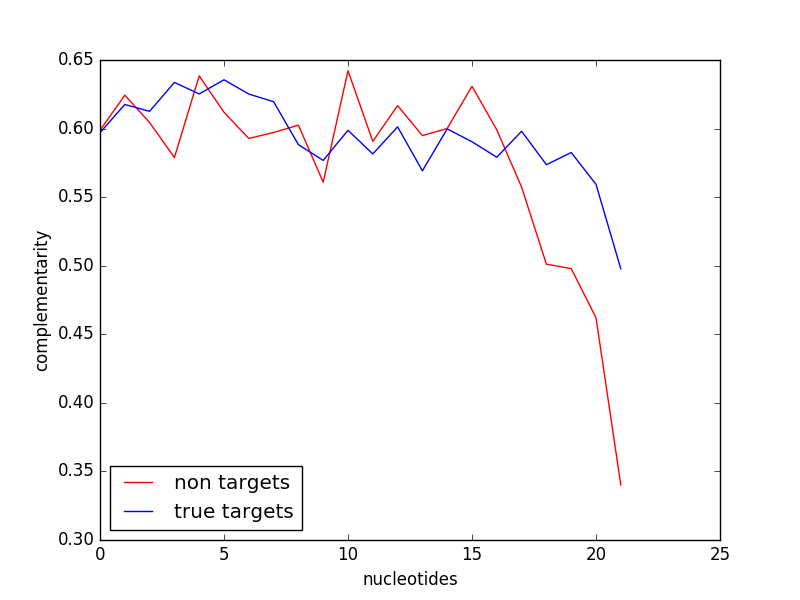
\includegraphics[scale=0.3]{results/curves-5-1_new.png}
\caption{Curves of complementarity of non and true targets: 1 -2 -2 -1, 5 -4 -6 -4 and -5 -1}
\label{curves}
\end{figure}


\begin{figure}
\hspace{-1cm}
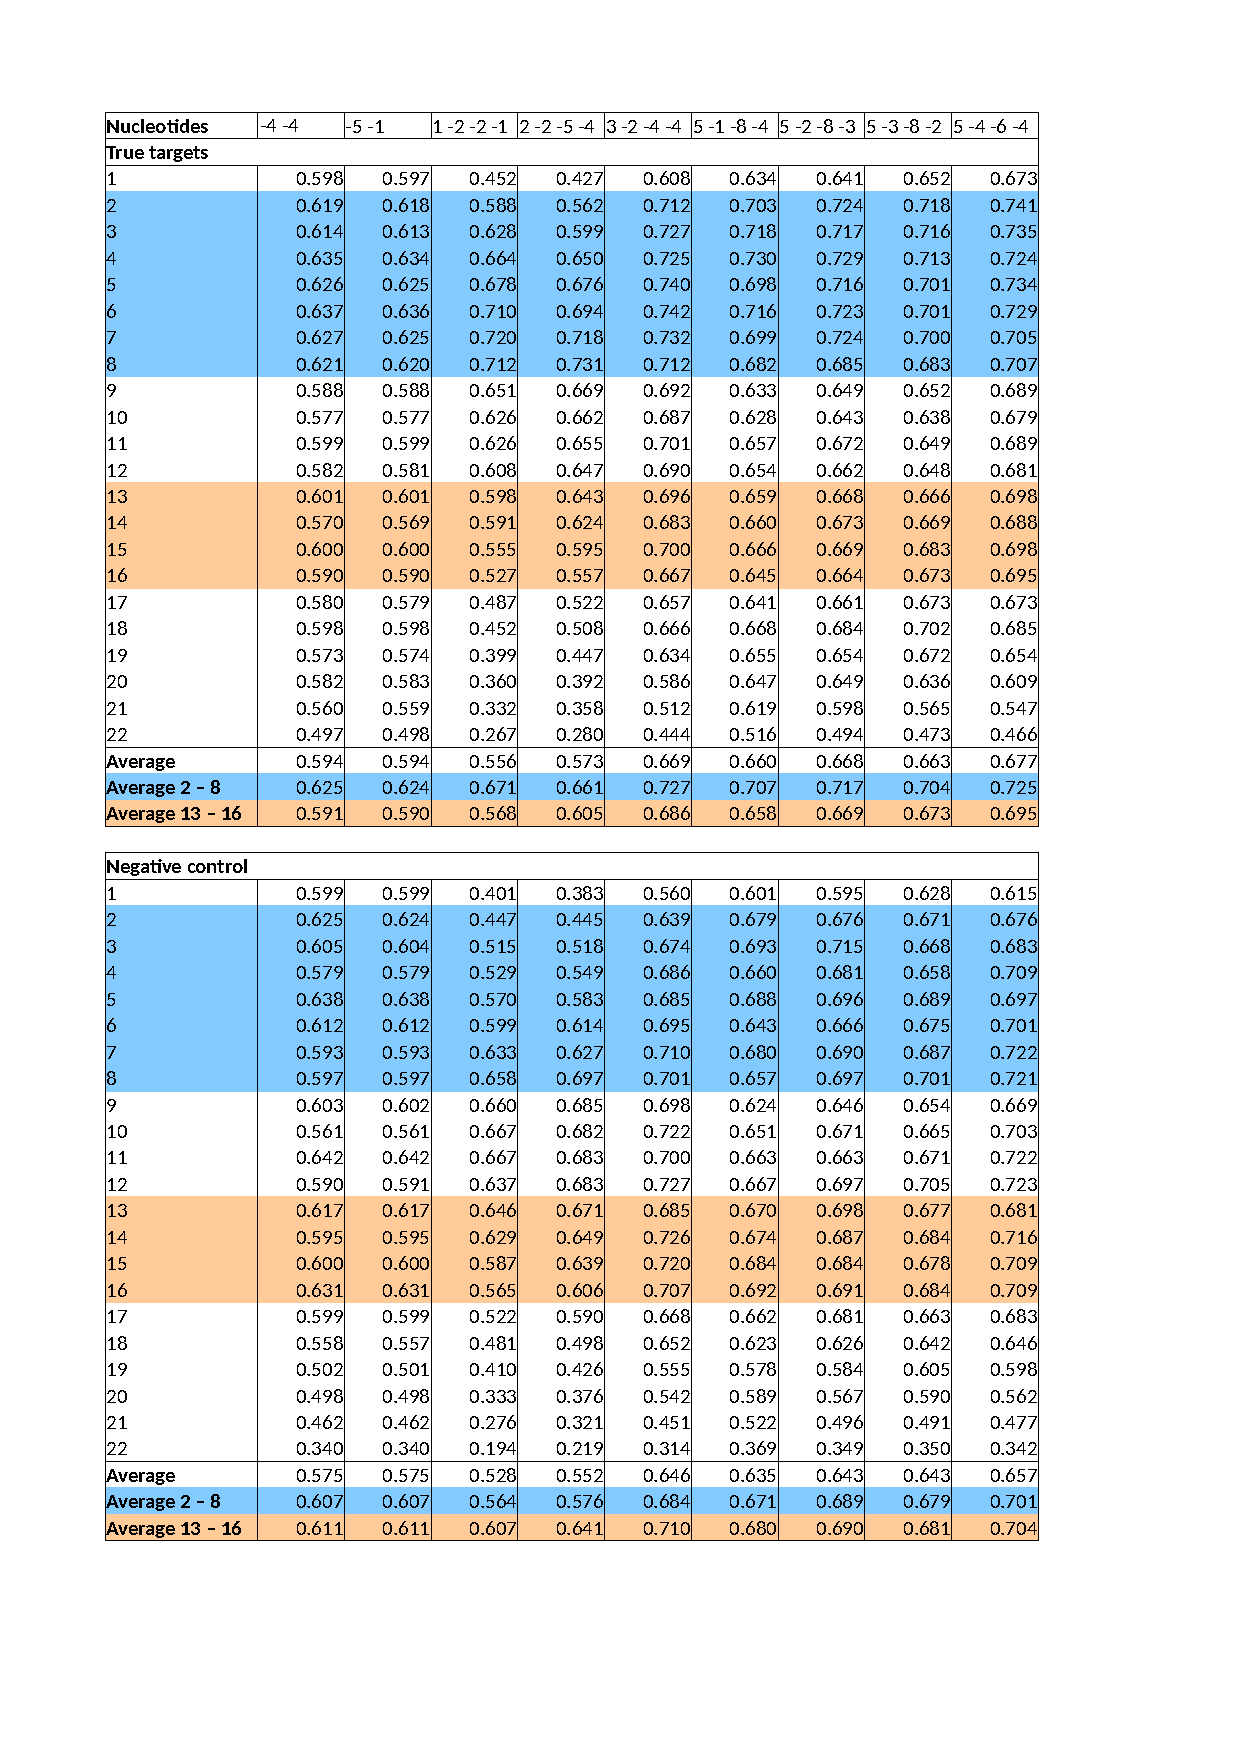
\includegraphics[scale=0.78]{results/ratio_table2.pdf}
\vspace{-3.1cm}
\caption{Table of ratios of complementarities}
\label{table:ratios}
\end{figure}



The table in figure~\ref{table:ratios} shows that the average of the complementarity ratios are similar when comparing true targets with non-targets. The nucleotides of the seed region are highlighted in blue and the ones of the additional 3' pairing in orange. Calculating the average complementarity ratios of these positions sheds light on the presence of these regions in validated interactions. For the first parameter set, the true targets show a small increase in the seed region but a decrease in the additional pairing. This feature of additional pairing can not be significantly observed. For the same set and its negative control, a constant average can be seen. Almost all true targets show an increase in the seed region and a decrease in the other region. For the non-targets there are different patterns. For example, for the third parameter set both regions increase compared to the standard average. For the other sets there is either no big difference or both increase but never decrease. Referring to the plots, the seed region in the true targets is slightly more visible than for the non-targets. All in all, the differences are not very big and significant. Both regions cannot be observed as clear as expected.  \\

The analysis of the alignment starting positions was not particularly successful and significant. Table~\ref{tab:positions} shows the numbers of the own predicted positions that were also given in the miRTarBase. It can be seen that two sets deliver only half the number of the other (5 -2 -8 -3 and 5 -3 -8 -2). These two sets also use very similar parameters. That shows that the alignment positions strongly depend on the selected parameters. In comparison to the given number of about 3700 positions in the miRTarBase, the numbers of the respective own found ones are in general not very high. Only about 20\% were found. This can be due to the different sizes of the UTRs of the genes. In this research the UTRs are from the UCSC website whereas the miRTarBase might use another source. Therefore the sizes can be a bit different resulting in different defined positions, although the alignment would start at the same position. To eliminate these small deviations, I allowed a window of 10 positions where the starting position can be. So if the provided miRTarBase position is given, the own predicted position is classified as consistent with the provided one if the position lies in a window of +5 or -5 related to the miRTarBase position. Another point is the difference that I align the miRNA sequence to the whole gene sequence. The best alignment position can therefore lie within the other region whereas the positions of the miRTarBase are only in the 3' UTR. If I only allow the 3' UTR, the number of consistent ones would be higher. Another reason for the inconsistent positions might be, that the tools they used in miRTarBase use better and more specific alignment tools where more parameters can be defined. The tools can better be adapted to a biological background like seed region and additional 3' pairing. The pairwise2 module only has 4 scoring parameters to select and only delivers the alignment with the highest score and no ranking.  \\



\begin{table} [h]
\caption{Number of common alignment starting positions}
\vspace{0.3cm}
\begin{tabular}{c||c|c|c|c|c} 
& 3 -2 -4 -4 & 5 -1 -8 -4 & 5 -2 -8 -3 & 5 -3 -8 -2 & 5 -4 -6 -4  \\
\hline\hline
Found number & 815 & 804 & 388 & 411 & 800\\
\hline
\end{tabular}
\vspace{0.5cm}

\begin{tabular}{c||c|c|c|c}
& 1 -2 -2 -1 & 2 -2 -5 -4 & -4 -4 & -5 -1 \\
\hline\hline
Found number & 882 & 793 & 776 & 845  \\
\hline
\end{tabular}
\label{tab:positions}
\end{table}






\chapter{Discussion}
\label{chapter:discussion}

The main focus in this research was on sequence alignment of miRNA sequence and its target mRNA sequence for given validated miRNA target interactions. This alignment should simulate a binding between the two sequences. With this method, it was investigated how this approach can be used to predict new target sites for miRNAs without any other biological experiments.\\

The results showed that with this alignment tool, the increase in the alignment score for true targets is significant. This means that if a certain threshold for the scoring is exceeded, with a certain error rate a considered mRNA is truly targeted by this miRNA. However, the p-values are extremely low, which is very surprising. Considering the existing tools, they always take many features into account to make the prediction more reliable. Therefore, considering this one single feature can not be as significant as the p-values express.\\

The other part of the analysis, the analysis of the complementarities, did not show significant differences between true targets and non-targets. The ratio of complementary nucleotides of miRNA and mRNA of true targets were not significantly higher than the ones of the non-targets. This means, the alignment did not detect better binding sites for the true targets regarding complementarity. According to the p-value and the alignment scores, the alignment of the true targets was better and had more matches and less mismatches or gaps. This however, can not be observed from the plots very well. Considering only the complementarity without the alignment scores, no statement about the probability of a true target can be made. Additionally, the seed region and the additional 3' pairing, which should be present in binding sites, were not detected. Small increases in the first few nucleotides could be observed but not as clearly as expected. This may be due to the unspecific alignment tool. It finds the best alignment position concerning the whole miRNA sequence. Therefore it does not set value on any special regions.  \\

Another problem is that with this alignment tool different binding sites were found compared to binding sites predicted by some existing prediction tools like miRanda. Whether the positions I found with the alignment tool are the right ones is questionable. The alignment strongly depends on parameters which leads to the difference in results. Surprisingly, the parameter set with similar parameters to miRanda was one of the sets where the fewest consistent positions were found. As mentioned above one reason for the low number of consistent positions can be varying used databases which can differ from each other in terms of sequence sizes. A big disadvantage of the Biopython module is that it only delivers the best alignment and not for example the best three. Additionally, I considered the whole gene sequence as a target. If the best alignment was found in other regions than the 3' UTR, the starting position can not be found in the miRTarBase. In these cases, additional alignments with high scores would be helpful to analyse if for example the second best alignment score is the one that is also provided in the miRTarBase. Another limitation of the module is the small potential to adjust the parameters to the given problem. \\

Nevertheless the scores showed a significant increase for the true targets. Yet, it is questionable how reliable this prediction feature is if considered on its own. As can be observed for the existing tools, a much better prediction is achieved when considering more prediction features as described below.\\

A first step can be the improvement of the alignment process, especially the refinement of the alignment parameters. In some other tools, like miRanda, the parameters are adapted to the binding mechanism. For example, in the present seed region the complementarity should be nearly perfect, meaning mismatches in the first few nucleotides should be highly penalized or only a certain number of mismatches should be allowed. In addition, mismatches or gaps in the central nucleotides of the miRNA can be present and are therefore not much penalized. Adapting the parameters to some targeting rules can highly improve the target prediction. A more general improvement is that the more data of true targets is available, the more can be learned from the mechanism and the more the prediction tools can be adapted in different ways concerning features and precision of features.\\

The complexity of the prediction is highlighted when considering the consensus of all predicted targets of the different tools. Only a really small subset of all targets are predicted by all tools. Further, comparing validated target interactions of the database with the results of all tools, about 16\% of all interactions are predicted by at least one tool. But there is no interaction that is predicted by all tools. That shows that there are big differences between the different tools partly because of the variable features they consider \cite{Keller}.\\ 

Because of their potential to function in treatment and detection of diseases, miRNAs become more and more important. Therefore miRNA research must be further extended and the complex target prediction has to be improved. Many researchers have found different additional features that can be considered. As described in the introduction, the seed region is one of the most important ones. The different types of sites vary in the effectiveness of repression. Grimson et al. (2007) investigate the different types and figure~\ref{types} shows their results. If one 8mer site is present, the repression effect is the highest \cite{Grimson}. \\


\begin{figure}[h]
\centering
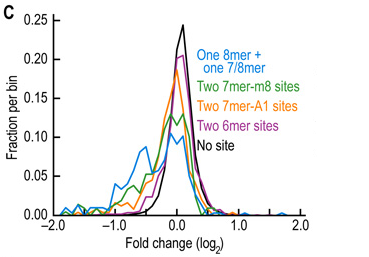
\includegraphics[scale=0.7]{results/site_3addi.png}
\caption{Effectiveness of different types of sites}
\label{types}
\end{figure}

Another useful feature is the free energy of the binding complex. This energy determines the stability and tightness of a  system, in this case the binding \cite{Peterson}. If the free energy is lower, the binding between the miRNA and mRNA is tighter resulting in more evidence that the miRNA actually targets this mRNA. If the energy is high then the binding is not very favourable, meaning the miRNA not favours to target this mRNA at this position. Some tools like RNAhybrid rely strongly on this feature \cite{Rehmsmeier}. \\

A completely different feature, the evolutionary conservation, can be taken into account. If a sequence occurs across species, it is defined as conserved. This implies that this part has been maintained by evolution because of a selected function \cite{Peterson}. Conservation near the miRNA binding site can indicate that this part of the sequence is necessary for some mechanisms. This includes conservation of the miRNA itself as well as the conservation of the respective site of the mRNA. These conservations can be analysed with phylogenetic methods. Figure~\ref{conserved} shows how conserved the different nucleotides of a miRNA are, indicating regions like the seed region and additional 3' pairing. \\

Site accessibility is a feature that Kertesz et al. (2007) investigated for their target prediction. The mRNA generally folds into a secondary structure. Therefore the miRNA cannot easily bind to its target because at first, interactions within the mRNA have to be broken to make the target accessible. As a result, miRNA will favourably bind to regions where the mRNA is more accessible. The researchers found that if the targets form stem structures, the repression is reduced. If sites occur in open loop structures, the repression is much higher. Summing up they found that site accessibility is not less important than seed matching \cite{Kertesz}. \\

As already mentioned above, in addition to the seed matching towards the 5' end, another complementary site towards the 3' end in the miRNA is present (Figure~\ref{addipairing}). Grimson et al. (2007) investigated that the highest down regulation was found when the site started at position 13 and had four or five contiguous base pairings (Figure~\ref{siteregulation}) \cite{Grimson}. Considering again the conservation of the nucleotides they found that outside the seed region the contiguous nucleotides starting from nucleotide 12, 13 or 14 were the most conserved ones indicating their functional importance (Figure~\ref{conserved}). Putting the information of seed region and additional base pairing together, it can be observed, if one 7mer-m8 site is present as well as a good 3' pairing, the efficacy is the highest. This is observed even though the difference between the efficacy of the presence of one 8mer site and the one mentioned before is not very big. But the improvement of the presence of a good 3' pairing instead of a poor one is more significant (Figure ~\ref{efficacy}). Between the two complementary areas there is usually a part of non-pairing nucleotides where bulges and mismatches are found. These are important for the prevention of the AGO cleavage function \cite{Filipowicz}.\\

\begin{figure}[h]
\centering
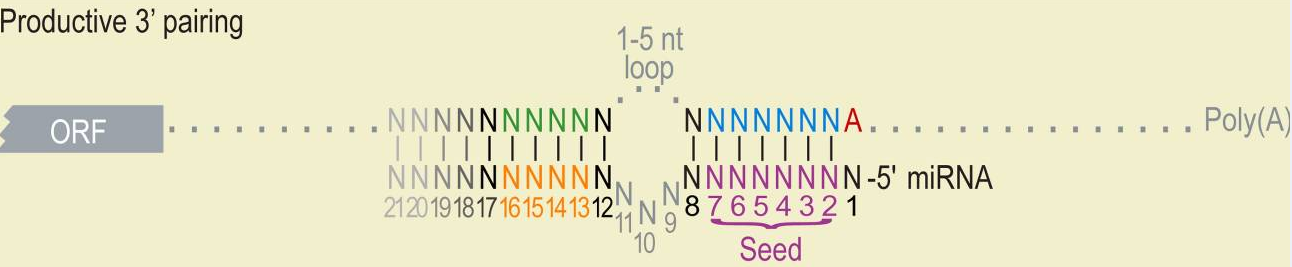
\includegraphics[scale=0.4]{results/additional_pairing.PNG}
\caption{Additional 3' pairing}
\label{addipairing}
\end{figure}

\begin{figure}[h]
\centering
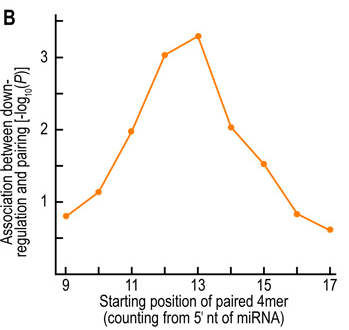
\includegraphics[scale=0.6]{results/sites_regulation.PNG} 
\caption{Relation between regulation and starting position of additional pairing}
\label{siteregulation}
\end{figure}

\begin{figure}[h]
\centering
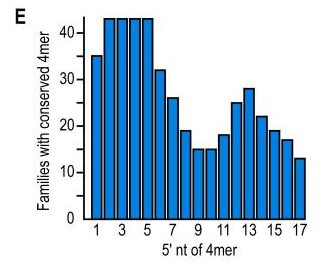
\includegraphics[scale=0.65]{results/sites_conserved.PNG} 
\caption{Conservation of nucleotide positions of miRNA}
\label{conserved}
\end{figure}

\begin{figure}[h]
\centering
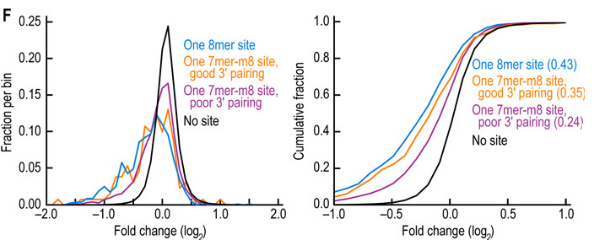
\includegraphics[scale=0.7]{results/site_efficacy.PNG} 
\caption{Efficacy of different combinations of seed region and additional 3' pairing}
\label{efficacy}
\end{figure}



To get an even more reliable and precise prediction even more features can be considered. The presence of GU-wobbles is common in targeting. In this wobble positions Guanine(G) binds to Uracil(U) even though the pairing with Cytosine would be prevalent. This special pairing is thermodynamically favourable. Therefore it occurs in many target interactions but also results in lower repression of the translation \cite{Doench}. As mentioned before, miRanda uses different scores for matches in the alignment step. They score the usual base pairing A-U and G-C with +5 and they penalize the other mismatches with a score of -3, excluding the pairing of G and U. This pairing is rewarded with at least +2 and therefore the GU wobbles are not penalized as much as other mismatches because they are very common \cite{Enright}. \\

Enright et al. (2003) and Doench et al. (2004) also found that the presence of multiple miRNA target sites results in a higher repression and destabilization of the mRNA. Grimson et al. (2007) further investigated that the distance between two sites is also an important criterion. Generally the repression of two present sites is the multiplication of the two single ones because they act independently. What is interesting is that if the two sites are adjacent, the repression is increased and not equal to the multiplication of the single ones. The increase in repression is however not very high (Figure~\ref{sitedistance}). To investigate the effect of cooperative miRNAs they analysed a mixture of miR-1 and miR-133 and simulated three different spacings. The results show that a spacing of four nucleotides did not show a cooperative repression but six or eight nucleotide spacing showed an increase in repression (Figure~\ref{sitespacing}). \\


\begin{figure}[h]
\centering
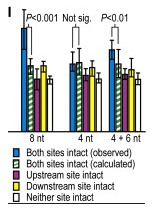
\includegraphics[scale=0.6]{results/sites_8nt.PNG}  
\caption{Cooperative repression with different site spacings}
\label{sitespacing}
\end{figure}

\begin{figure}[h]
\centering
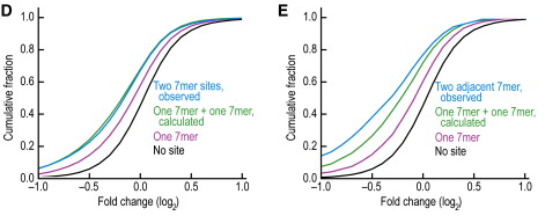
\includegraphics[scale=0.65]{results/sites_distance.PNG}
\caption{Effect of multiple sites}
\label{sitedistance}
\end{figure}

Another indicator is the position of the binding site relative to the stop codon and the center of the UTR. Generally sites in the 3' UTR are investigated but Grimson et al. (2007) detected that sites in the Open reading frame (ORF) are slightly effective, sites in the 5' UTR not at all. Figure~\ref{siteorf} shows the different efficacies regarding the site location. Another characteristic concerning the site locations is the distance from the stop codon. Figure~\ref{sitestop} illustrates that approximately in the first 15 nucleotides the efficacy is still very low like in the ORF but afterwards it increases a lot. The sites were present at least 15 nucleotides from the stop codon and not present in the center of long UTRs. \\

\begin{figure}
\centering
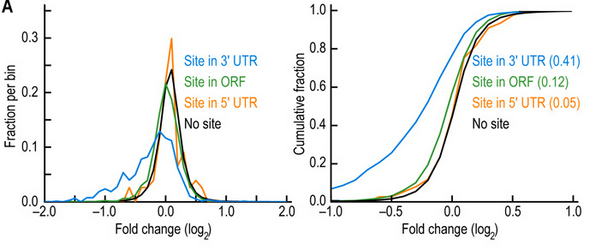
\includegraphics[scale=0.74]{results/sites_orf.PNG}
\caption{Efficacy of different site locations}
\label{siteorf}
\end{figure}

\begin{figure}
\centering
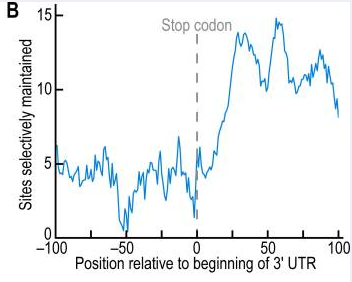
\includegraphics[scale=0.6]{results/site_stop.PNG} 
\caption{Efficacy of sites located relative to the stop codon}
\label{sitestop}
\end{figure}


   
Considering all these different common and less common features, new targets for miRNAs can be predicted more reliably. Figure~\ref{fig:tools} shows known prediction tools and the features they consider. As mentioned above the most common feature that nearly all of them consider are seed matching, conservation and free energy. \\


\begin{figure}
\centering
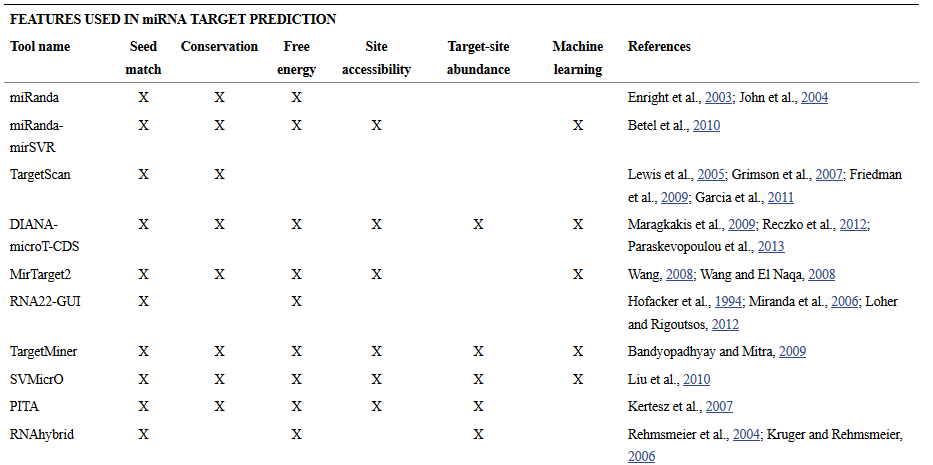
\includegraphics[scale=0.6]{results/tools.PNG}
\caption{Prediction tools and their features}
\label{fig:tools}
\end{figure}


\vspace{2cm}



\chapter{Conclusion}
\label{chapter:conlusion}

The research showed that, according to the p-values, the consideration of the sequence alignment scores is already significant. Nevertheless, the prediction still includes many errors. To improve the prediction many other features should be considered.
As described above, there are a lot of features that can be taken into account as well as many different tools already exist. They all differ from each other in the number and type of features they use and also in the weighting of the single features \cite{Peterson}. Concluding, each tool and feature has its advantages and strengths but also its limitations which makes none of the existing tools perfect and 100\% reliable. Relying on just a few features will for sure lead to many errors, either false positives or false negatives. There are many irregularities and some features like the free energy are not always very precise \cite{Peterson}. These problems have to be incorporated to lower the error rate.\\

Additionally not every tool is frequently updated which is a big problem and does not lead to improvements in target prediction. Some tools do not use the current data or innovations in target interactions. According to Peterson et al. (2014) the following tools are outstanding because of maintenance, newest input data and they are the easiest once to use: DIANA-microT-CDS, miRanda-mirSVR and Targetscan \cite{Peterson}. All three are somehow unique but all for example use looser thresholds for conservation allowing less conserved regions to balance irregularities and refuse less true targets.\\

The early miRanda tool is also still widely used. Its strengths are the optimization of the sequence complementarity. This is due to the specific rules and requirements for example regarding the sequeunce alignment and conservation. However, the tool permits imperfect bindings. Additionally, it emphasizes the presence of multiple binding sites in the 3' UTR, either of the same miRNA or of others. This might result in refusing miRNAs with only one site leading to many false positives \cite{John}. In contrast, TargetScan places emphasis on the seed region with its many different seed types and context scores. Having binding sites with less perfect seed regions even though they are functional, the tool would ignore them \cite{Lewis}. The last favoured tool, DIANA-microT-CDS, predicts only single binding sites, which can be conserved and non-conserved \cite{Kiriakidou}. Certainly, the presence of multiple binding sizes might result in weaker interactions that are therefore underestimated by this tool. However, with its signal to noise ratio, which evaluates the specificity, and the resulting prediction score, which correlates with the amount of produced protein, DIANA-microT-CDS is an innovative, successful prediction tool \cite{Maragkakis}. The class of tools, like miRSVR, learn how to weight the different features they consider with support vector regression \cite{Betel}. These machine-learning based approaches are getting more accurate the more positive and negative target data is verified and the more features are identified. Consequently, because of the lack of this data, these tools are not significantly better than other tools mentioned above \cite{Peterson}. \\

Fujiwara and Yada (2013) followed a new approach by considering other characteristics than binding sites for the prediction, such as the transcriptional regulation. In their research they searched for common cis-elements in the miRNA as well as in the target gene. Compared to conventional methods, their method is almost as good as the standard binding site based ones but combining the two different methods decreases the accuracy a lot. The advantages of this novel approach are independence of conservation of binding sites and the amount of available training data \cite{Fuji}. \\

Coronnello and Benos (2013) investigated another approach trying to improve the prediction power. They developed a tool, ComiR, that additionally considers the miRNA expression levels and the combination of miRNA bindings. It also combines different scoring schemes from tools mentioned above. The innovation in this tool is the investigation of sets of miRNAs and their co-expression \cite{Coronnello}. \\

All in all, the analysis of miRNAs is very complex and needs to be improved in terms of prediction. The future consists of elimination of the limits of some tools and finding more useful features for the prediction.



\bibliography{bachelor}


\listoffigures
\listoftables


%Figure~\ref{biogenesis}: \cite{Kelly} http://www.nature.com/nrurol/journal/v9/n7/images/nrurol.2012.104-f1.jpg
%Figure ~\ref{seed}: http://journal.frontiersin.org/article/10.3389/fgene.2014.00023/full

%Figure sites: http://www.ncbi.nlm.nih.gov/pubmed/17612493

%Table ~\ref{fig:tools}: http://www.ncbi.nlm.nih.gov/pmc/articles/PMC3927079/





\end{document}